\begin{figure}[!ht]
\centering
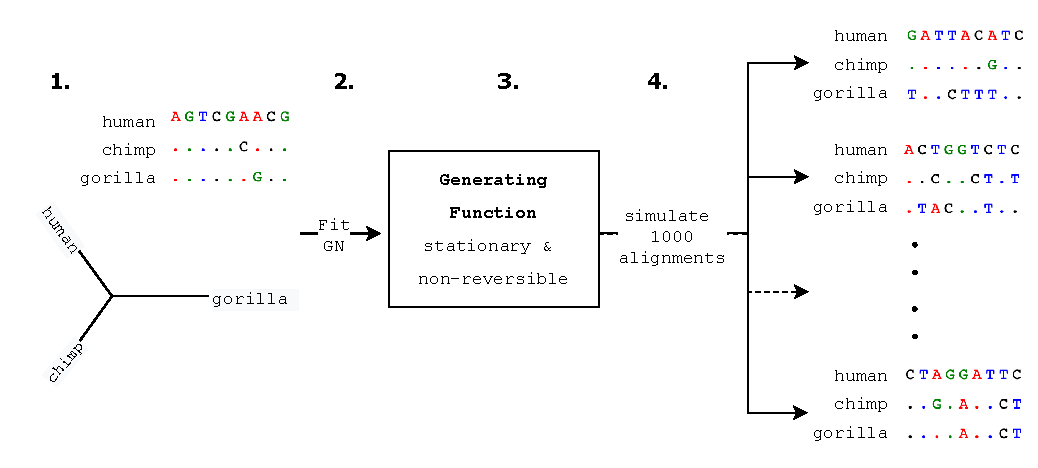
\includegraphics[width=\textwidth]{figures/simulating_alns.pdf}
\caption{Creating synthetic data sets whose evolution was stationary but not reversible. \textbf{1,} select seed alignment, \textbf{2}, fit GN mixed model and extract model parameter estimates, \textbf{3}, define generating function using parameter estimates altered to be stationary, \textbf{4}, generate 1000 alignments of length $n$ and branch length scaled by $b$. For all 4 seeds this was performed for n = 300, 3000, 30000, and for each n, b = 1 and 3.}
\label{fig:simulating_alns}
\end{figure}